\documentclass[a4paper,12pt,oneside]{book} % nie: report!


% pakiety
\usepackage{polski} % lepiej to zamiast babel!
\usepackage[utf8]{inputenc} % w razie kłopotów spróbować: \usepackage[utf8x]{inputenc}
\usepackage{fancyhdr} % nagłówki i stopki
\usepackage{indentfirst} % WAŻNE, MA BYĆ!
\usepackage[pdftex]{graphicx} % to do wstawiania rysunków
\usepackage{amsmath} % to do dodatkowych symboli, przydatne
\usepackage[pdftex,
            left=1in,right=1in,
            top=1in,bottom=1in]{geometry} % marginsy
\usepackage{amssymb} % to też do dodatkowych symboli, też przydatne
\usepackage{pdfpages}
\usepackage{lipsum}
\usepackage{multirow}
\usepackage{listings}
\usepackage{caption}
\usepackage{booktabs}
\usepackage{subcaption}
\usepackage{xcolor}
\graphicspath{ {./img/} }
\DeclareCaptionType{code}[Listing][Spis listingów] 

\definecolor{codegreen}{rgb}{0,0.6,0}
\definecolor{codegray}{rgb}{0.5,0.5,0.5}
\definecolor{codepurple}{rgb}{0.58,0,0.82}
\definecolor{backcolour}{rgb}{0.95,0.95,0.92}

\lstset{
	backgroundcolor=\color{backcolour},   
	commentstyle=\color{codegreen},
	keywordstyle=\color{magenta},
	numberstyle=\tiny\color{codegray},
	stringstyle=\color{codepurple},
	basicstyle=\ttfamily\footnotesize,
	breakatwhitespace=false,         
	breaklines=true,                 
	captionpos=b,                    
	keepspaces=true,                 
	numbers=left,                    
	numbersep=5pt,                  
	showspaces=false,                
	showstringspaces=false,
	showtabs=false,                  
	tabsize=2,
	float=h
}

% definicje nagłówków i stopek
\pagestyle{fancy}
\renewcommand{\chaptermark}[1]{\markboth{#1}{}}
\renewcommand{\sectionmark}[1]{\markright{\thesection\ #1}}
\fancyhf{}
\fancyhead[LE,RO]{\footnotesize\bfseries\thepage}
\fancyhead[LO]{\footnotesize\rightmark}
\fancyhead[RE]{\footnotesize\leftmark}
\renewcommand{\headrulewidth}{0.5pt}
\renewcommand{\footrulewidth}{0pt}
\addtolength{\headheight}{1.5pt}
\fancypagestyle{plain}{\fancyhead{}\cfoot{\footnotesize\bfseries\thepage}\renewcommand{\headrulewidth}{0pt}}


% interlinia
\linespread{1.25}


% treść
\begin{document}
\sloppy
\thispagestyle{empty}

\includepdf{stronatytulowa}
\newpage{}

\thispagestyle{empty}
\newpage{}

\tableofcontents{}

\chapter*{Wstęp}
\addcontentsline{toc}{chapter}{Wstęp}
\label{Wstep}
%Mega ogólne sprawy dotyczące tego co chce zrobić
Sieci neuronowe mają za zadanie naśladowanie zachowań sieci neuronów znajdujących się w mózgu człowieka. Zostały stworzone do rozwiązywania zadań trudnych lub prawie niemożliwych do opisania za pomocą reguł, wyrażeń logicznych i innych narzędzi programistycznych. Wraz z rozwojem sieci neuronowych powstało wiele wariantów, które ze względu na swoją budowę lepiej lub gorzej sprawdzają się w różnych problemach. W przypadku rozpoznawania obrazów w postaci dwu-wymiarowej macierzy dla danych monochromatycznych lub trój-wymiarowej macierzy dla zdjęć kolorowych jednym z najlepszych wyborów będą sieci konwolucyjne. Sieci te rozpoznają wzorce, poczynając od linii horyzontalnych i wertykalnych, a w dalszych warstwach kończąc na skomplikowanych strukturach. Budowa i działanie sieci konwolucyjnych daje wielki potencjał do klasyfikacji obrazów. Niniejsza praca licencjacka przedstawia przykład wieloklasowej klasyfikacji tj. rozpoznawania liter alfabetu ASL przy wykorzystaniu sieci konwolucyjnych.

\chapter*{Cel i zakres pracy}
\addcontentsline{toc}{chapter}{Cel i zakres pracy}
\label{Cel i zakres pracy}
%celem pracy jest napisanie programu bla bla
Celem pracy jest stworzenie programu wyposażonego w wytrenowany model do rozpoznawania obrazu, który w czasie rzeczywistym używając kamery internetowej będzie w stanie odczytać i wyświetlić na ekranie transkrypcję znaków języka migowego pokazywanych przez osobę znajdującą się w polu widzenia kamery. Dodatkowo, w celu osiągnięcia celu pracy, zrealizowano następujące zadania: utworzenie zbioru danych składającego się z około 50000 zdjęć zawierających wszystkie litery alfabetu ASL, utworzenie modelu z warstw konwolucyjnych i gęstych oraz wytrenowanie modelu i tuning parametrów. W teoretycznej części pracy przybliżono temat języka migowego American Sign Language, jak również temat konwolucyjnych sieci neuronowych i sposobu działania modeli.

\chapter{Język migowy American Sign Language}
American Sign Language (Amerykański Język Migowy, ASL) to złożony język wizualno-przestrzenny używany przez osoby niesłyszące w Stanach Zjednoczonych Ameryki oraz anglojęzycznych częściach Kanady. Jest to w pełni kompletny język naturalny. ASL jest językiem natywnym dla wielu mężczyzn, kobiet i dzieci, a także niektórych słyszących dzieci w rodzinach, gdzie opiekunowie prawni są niesłyszący \cite{nakamura}.
\section{Historia}
Pochodzenie dzisiejszej społeczności osób niesłyszących w Stanach Zjednoczonych jest powszechnie utożsamiane z założeniem pierwszej szkoły dla niesłyszących - American School for the Deaf (ASD), założonej w 1817 roku w Hartford, Connecticut. Przed założeniem szkoły ASD na terenie USA działało wiele niezależnych społeczności, poczynając od małych grup o wielkości pojedynczej rodziny do większych - całych wsi. W małych społecznościach uformowały się niezależne znaki i systemy języka migowego, które są obecne po dziś dzień w tych środowiskach. Istnieją dowody na to, że niesłyszące dzieci kształtowały swoje własne systemy języków migowych, które były o wiele bardziej wyrafinowane od tych, używanych w społeczności, w których się znajdowały \cite{bahan}.

Istnieją również doniesienia o innym niezależnie uformowanym systemie języka migowego Martha’s Vineyard Sign Language (MVSL), który istniał przed założeniem American School for the Deaf. Język ten był głównie używany w wsi Chilmark na wybrzeżu Massachusetts. Powstanie MVSL zapoczątkował fakt, że wspomniana społeczność Chilmark miała wysoki odsetek mutacji genetycznych prowadzących do głuchoty. W skali miasteczka około 4 procent mieszkańców było niesłyszących. Wynikało to z wysokiego odsetka mieszanych małżeństw od wielu pokoleń, począwszy od hrabstwa Kent w Angli, zanim wieś Chilmark została założona w roku 1690 \cite{groce}. Mieszkańcy, którzy nie byli niesłyszący również posługiwali się językiem MVSL, wówczas gdy znajdowali się w towarzystwie osób z niepełnosprawnością ale również, gdy w gronie rozmówców nie było osoby niesłyszącej. Język był używany do czasu założenia szkoły dla osób niesłyszących ASD w Hartford. Dzieci z wsi Chilmark zaczęto wysyłać do szkoły American School for the Deaf we wczesnych latach dwudziestych XIX wieku. Skutkowało to zatarciem się języków MVSL i nowego języka migowego ewoluującego w dzisiejszy język ASL \cite{bahan}.

Kiedy szkoła dla niesłyszących została założona, stała się miejscem, gdzie wiele pomniejszych systemów migowych stykało i mieszało się ze sobą przez 175 lat. Z mieszanki tych języków powstał dzisiejszy język ASL. Niesłyszący nauczyciel - Laurent Clerc, pochodzący z Francji, był pierwszym nauczycielem w wspomnianej placówce. Z kraju swojego pochodzenia przywiózł wiedzę o Francuskim Języku Migowym, którego znaków nauczał w amerykańskiej szkole. Ta sytuacja spowodowała bardzo mocne doprawienie wówczas powstającego języka ASL o aspekty zaciągnięte z Francuskiego Języka Migowego. Na dzień dzisiejszy około 60 procent współczesnego systemu ASL opiera się na starym migowym języku Francuskim \cite{bahan}.


\section{Populacja}
Informacje dostępne w internecie nie dają jednoznacznej odpowiedzi na pytanie - ile osób używa języka ASL. Wyszukane rezultaty są bardzo niejednoznaczne \cite{population}.
\begin{table}[h!]
	\caption{Szacowane rankingi użytkowników ASL według różnych źródeł}
	\resizebox{\textwidth}{!}{
	\begin{tabular}{@{}ll@{}}
			\toprule
			\textbf{Oszacowany ranking} & \textbf{Źródło} \\ \toprule
			100,000 – 500,000 & 
			\begin{tabular}[c]{@{}l@{}}
				ERIC Digests (Wilcox \& Peyton, 1999) \\ MSN Encarta (Wilcox, 2004) \\ Ethnologue.com (Ethnologue, 2004) 
			\end{tabular}\\\\
	
			250,000 – 500,000 & 
			\begin{tabular}[c]{@{}l@{}}
				\parbox{16cm}{American Sign Language Program @ The University of Iowa (Department of Speech Pathology and Audiology, 2004)} \\
				\parbox{16cm}{ASLTA (NC ASLTA and NCAD Ad Hoc Committee, 2004)} \\
				\parbox{16cm}{Colorado Department of Human Services (Colorado Commission for the Deaf and Hard of Hearing, n.d.)}
			\end{tabular}\\\\
			300,000 – 500,000 & 
			\begin{tabular}[c]{@{}l@{}}
				\parbox{16cm}{Barnes\&Noble.com (Costello, 1994)} \\
				\parbox{16cm}{SignWriting.org (Rosenberg, 1999)}
			\end{tabular}\\\\
			500,000 & 
			\begin{tabular}[c]{@{}l@{}}
				\parbox{16cm}{American Academy of Family Physicians (CDGAP, 1997)} \\
				\parbox{16cm}{ASLinfo.com (ASLinfo.com, n.d.)} \\
				\parbox{16cm}{DEAF C.A.N.! (Deaf Community Advocacy Network, n.d.)}
			\end{tabular}\\\\
			500,000 – 2,000,000 & 
			\begin{tabular}[c]{@{}l@{}}
				\parbox{16cm}{Brenda Schick, Ph.D. (Schick, 1998) } \\
				\parbox{16cm}{DawnSignPress (DawnSignPress, 2003) } \\
				\parbox{16cm}{Gallaudet University Library (Harrington, 2004)}
			\end{tabular}\\\\
			15,000,000 & 
			\begin{tabular}[c]{@{}l@{}}
				\parbox{16cm}{Aetna InteliHealth (Gordon, 2001) }
			\end{tabular}\\\\
			\begin{tabular}[c]{@{}l@{}}
				3rd most used language \\ in the U.S.
			\end{tabular} & 
			\begin{tabular}[c]{@{}l@{}}
				\parbox{16cm}{HandSpeak (HandSpeak.com, n.d.) } \\
				\parbox{16cm}{Health Literacy Consulting (Osborne, 2003) } \\
				\parbox{16cm}{Missouri Office of State Courts Administrator (Office of State
					Courts Administrator, n.d.)}
			\end{tabular}\\\\
			
			\begin{tabular}[c]{@{}l@{}}
				4th most used language \\ in the U.S.
			\end{tabular}	 		& 
			\begin{tabular}[c]{@{}l@{}}
				\parbox{16cm}{The ASHA Leader Online (Scott \& Lee, 2003) } \\
				\parbox{16cm}{Deaf Resource Library (Nakamura, 2002) } \\
				\parbox{16cm}{NIDCD (National Institute on Deafness and Other
					Communication Disorders, 2000) }
			\end{tabular}\\ \\
			\begin{tabular}[c]{@{}l@{}}
				3rd to 10th most used \\ language in the U.S. 
			\end{tabular}	& Wikipedia (Wikimedia, 2003) \\ \bottomrule
		\end{tabular}
	}
	\label{tab:ratings}
\end{table}
Znalezione szacunkowe (Tabela \ref{tab:ratings}) liczby użytkowników języka ASL wahają się począwszy od 100 tysięcy do nawet 15 milionów. Warto zwrócić uwagę, że prawdopodobnie szacunki Aetna InteliHealth zostały omyłkowo utożsamione z użytkownikami języka ASL, a tak naprawdę mogą przedstawiać liczbę osób ze znacznym i całkowitym ubytkiem słuchu \cite{population}.

Starając się uogólnić wszystkie szacunki płynące ze źródeł internetowych, kształtują się dwa główne twierdzenia:
\begin{itemize}
	\item Jest mniej niż dwa miliony użytkowników ASL, ale bardziej prawdopodobne, że ta liczba jest mniejsza i wynosi mniej niż półtora miliona ludzi w Stanach Zjednoczonych Ameryki;
	\item ASL może być trzecim najczęściej występującym językiem w Stanach Zjednoczonych \cite{population}.
\end{itemize}

Zaprezentowane w tabeli \ref{tab:ratings} dane pochodzą głównie z okresu lat dwutysięcznych. W trakcie pisania niniejszej pracy prawdopodobnie nie istniały bardziej aktualne i ogólnodostępne źródła.

\section{American Manual Alphabet}
American Manual Alphabet to zbiór różnych gestów dłonią reprezentujący wszystkie litery angielskiego alfabetu. Są one ważnym elementem komunikacji i uzupełniają American Sign Language o zestaw znaków pozwalających na wyrażenie słów, dla których rozmówca nie zna konkretnego znaku lub nazw własnych, takich jak imiona czy nazwy firm. Często używane są przez użytkowników ASL dla upewnienia się, że idea tego co chcieli powiedzieć została dokładnie i zrozumiale zakomunikowana drugiej stronie rozmowy. Początkujący użytkownicy języka ASL, z racji ograniczonego zbioru znaków często posiłkują się alfabetem migowym do komunikowania słów, dla których nie znają odpowiadających znaków \cite{costello}.

\begin{figure}[h]
\centering
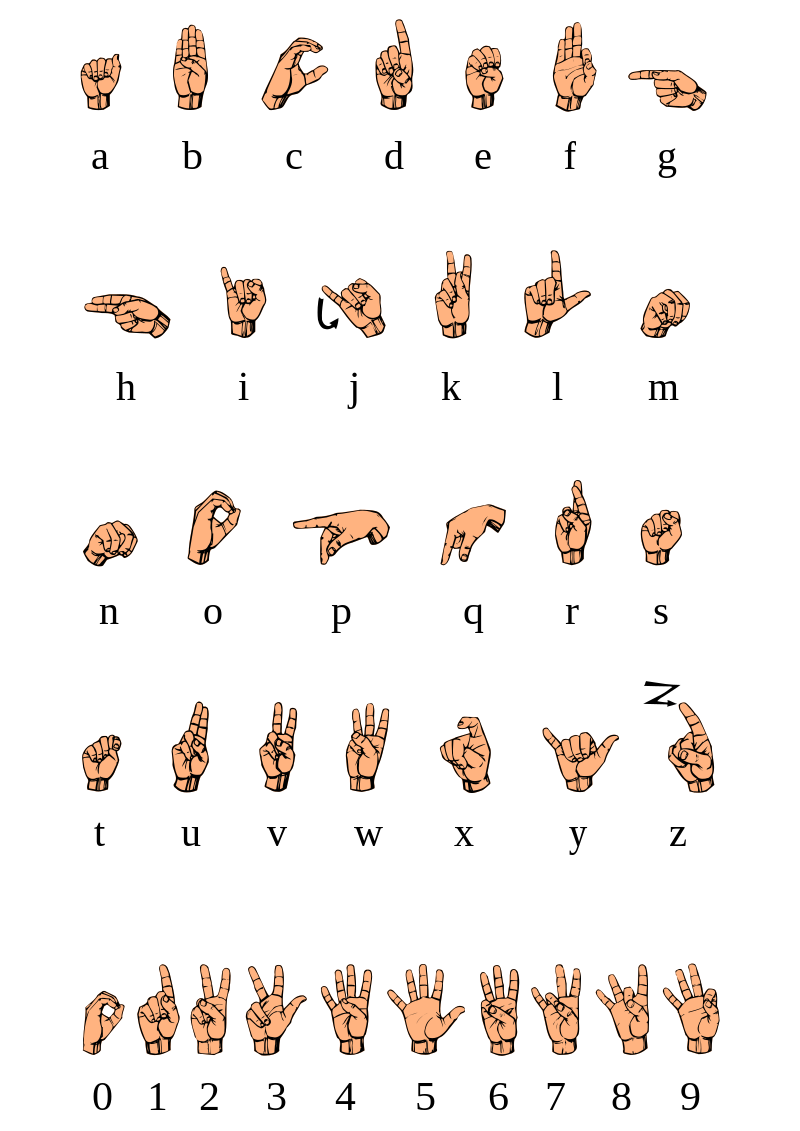
\includegraphics[scale=0.45]{ama.png}
\caption{American Manual Alphabet \cite{wikipedia_2022}}
\end{figure}

W alfabecie znajduje się 26 znaków odpowiadających literom języka angielskiego. Na odpowiedniki liter składa się 19 ułożeń dłoni. Niektóre ułożenia występują kilkukrotnie tak jak litery "i" i "j" oraz "p" i "k". Różnica pomiędzy tymi znakami polega na ruchu dłonią (przy literze "j" występuje ruch w kształcie półkola) lub pozycji względem ciała (przy literze "k" dłoń jest skierowana palcami do góry, a przy literze "p" w dół lub w bok) \cite{costello}.


\chapter{Konwolucyjne sieci neuronowe i rozpoznawanie obrazów}

Konwolucyjne sieci neuronowe pozwoliły na przełomowe osiągnięcia ostatniej dekady w dziedzinie rozpoznawania wzorców, zaczynając od obrazów a kończąc na rozpoznawaniu głosu. Jednym z wyróżników sieci CNN jest znaczna redukcja ilości parametrów w dalszej części modelu. Mniejsza ilość parametrów pozwoliła na budowanie większych sieci, które mogą rozwiązywać bardziej skomplikowane problemy niż dotychczasowe modele z użyciem zwykłych sieci neuronowych \cite{8308186}.

\section{Zasada działania sieci konwolucyjnych (CNN)}

Model CNN na swoim wejściu posiada najczęściej naprzemiennie ustawione warstwy konwolucyjne i Pooling. Pozwala to na automatyczne wykrywanie cech charakterystycznych i bardzo szybkie zmniejszenie objętości przetwarzanych danych. Przetworzone dane obrazu wejściowego są spłaszczane do jednego wymiaru przez warstwę Flatten. Spłaszczone dane przyjmują kolejne warstwy gęsto połączone i dokonują ostatecznej klasyfikacji danych wejściowych do danej kategorii \cite{9463236}.

Przykładowy model został przedstawiony na rysunku \ref{cnn_mod}.

\begin{figure}[h]
	\centering
	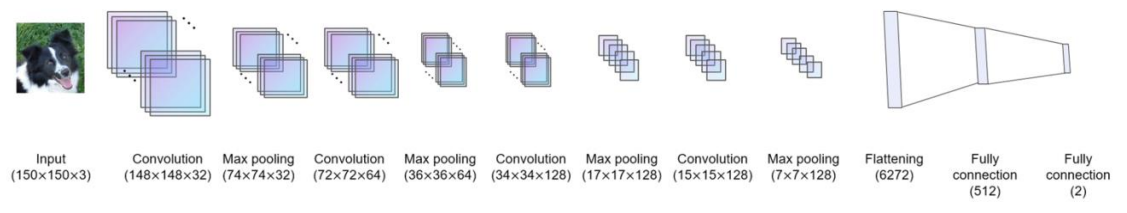
\includegraphics[scale=0.55]{cnn_arch.png}
	\caption{Model CNN \cite{cnnarch}}
	\label{cnn_mod}
\end{figure}

\section{Architektura CNN}

\subsection{Warstwy konwolucyjne}
\label{konw}

Warstwa konwolucyjna wykonuje prostą operację nałożenia filtra zachowującego się na wzór funkcji aktywacji (rys. \ref{conv_filter}). Przeprowadzenie tej operacji piksel po pikselu przez wiele filtrów tworzy mapy cech, które są później wykorzystywane w kolejnych warstwach modelu \cite{9388351}. Warstwy konwolucyjne zamiast pełnego połączenia, gdzie każdy piksel obrazu wejściowego jest połączony z każdym pikselem obrazu wyjściowego, stosuje lokalne pola recepcyjne zmniejszając drastycznie liczbę połączeń (rys. \ref{conv_img}).

\begin{figure}[h]
	\centering
	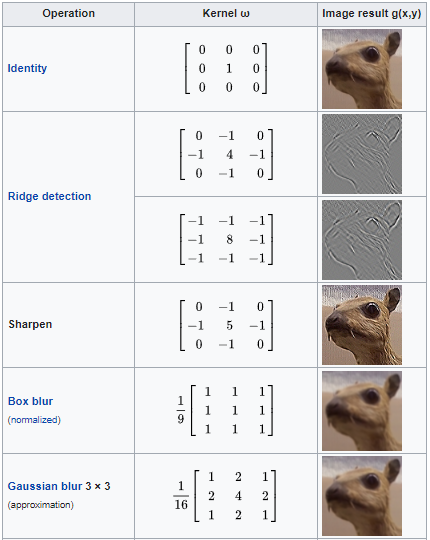
\includegraphics[scale=0.9]{conv_filter.png}
	\caption{Przykładowe działanie filtrów 3x3 na obrazach \cite{wikipedia_filterkernel}}
	\label{conv_filter}
\end{figure}

\begin{figure}[h]
	\centering
	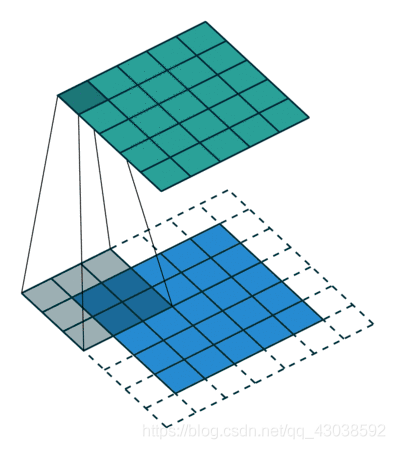
\includegraphics[scale=0.4]{conv.png}
	\caption{Warstwa konwolucyjna - zasada działania \cite{developpapercom_2021}}
	\label{conv_img}
\end{figure}

Warstwy konwolucyjne pozwalają na jeszcze większe zmniejszenie ilości parametrów. Mowa o opcji ustawienia skoku pomiędzy polami recepcyjnymi - \emph{stride}, które domyślnie zachodzą na siebie przy wartości parametru = 1. Po konfiguracji \emph{stride} możliwe jest częściowe lub całkowite rozdzielenie poszczególnych węzłów (rys. \ref{stride_img}) \cite{8308186}.

\begin{figure}[h]
	\centering
	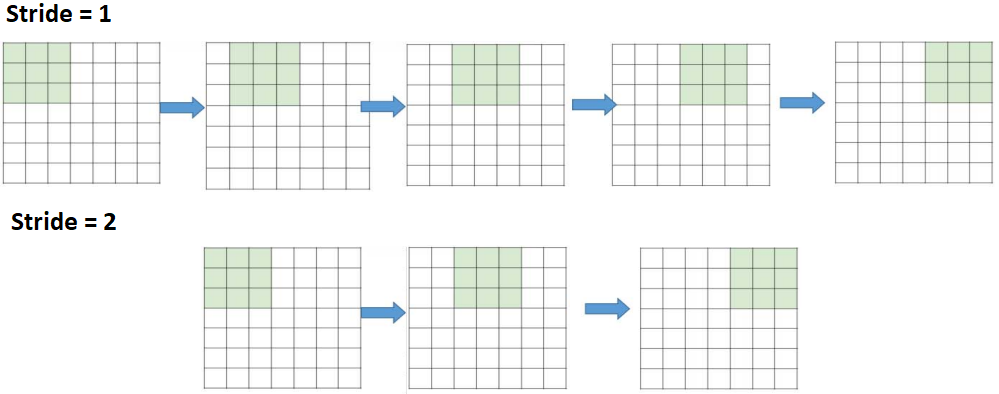
\includegraphics[scale=0.6]{stride.png}
	\caption{Różnica w odstępach pomiędzy polami recepcyjnymi w zależności od parametru \emph{stride} \cite{8308186}}
	\label{stride_img}
\end{figure}

Jedną z wad warstw konwolucyjnych jest utrata informacji, która pojawia się na obrzeżach obrazu. Istnieje bardzo prosta i efektywna metoda do rozwiązania tego problemu - \textit{"zero-padding"}. Zaletą takiego rozwiązania, jest również zachowanie rozmiaru obrazu na wyjściu warstwy. Dla przykładu (rys. \ref{no_padding}) z wartościami N=7, F=3 i parametrze \emph{stride}=1, rozmiar danych wyjściowych wyniesie 5x5, gdzie oryginalny rozmiar danych wejściowych wynosił 7x7 \cite{8308186}.

\begin{figure}[h]
	\centering
	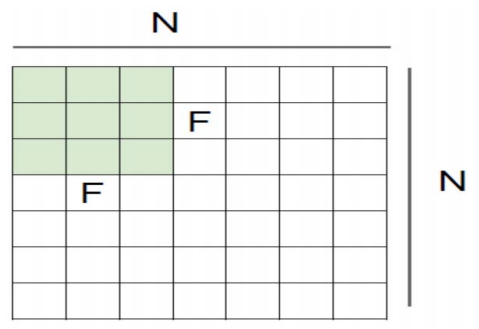
\includegraphics[scale=0.45]{no_padding.png}
	\caption{Dane bez zero-padding \cite{8308186}}
	\label{no_padding}
\end{figure}

Wzór na obliczenie rozmiaru wyjściowego obrazu \emph{O} dla danych wejściowych \emph{N x N} i rozmiarze filtra \emph{F x F}, jest następujący:
\begin{equation}
	O = 1 + \frac{N-F}{S}
	\label{nopaddingoutput}
\end{equation}
Gdzie:
\begin{itemize}
	\item N - rozmiar danych wejściowych,
	\item F - rozmiar filtra,
	\item S - wartość parametru \emph{stride}.
\end{itemize}


Natomiast, dodając wypełnienie zerami rozmiar danych wyjściowych będzie wynosił 7x7, taki sam jak danych wejściowych (rys. \ref{padding}) \cite{8308186}. 

\begin{figure}[h]
	\centering
	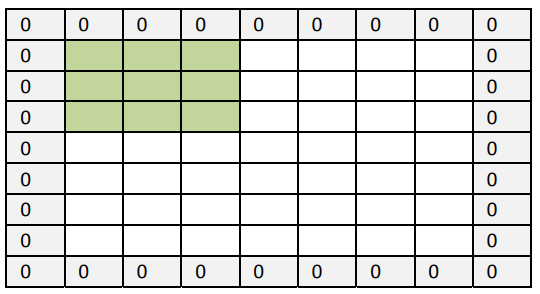
\includegraphics[scale=0.45]{padding.png}
	\caption{Dane z zero-padding \cite{8308186}}
	\label{padding}
\end{figure}

W przypadku uzupełniania zerami następuje lekka modyfikacja wzoru \ref{nopaddingoutput}:
\begin{equation}
	O = 1 + \frac{N+2P-F}{S}
	\label{paddingoutput}
\end{equation}
gdzie:
\begin{itemize}
	\item N - rozmiar danych wejściowych,
	\item F - rozmiar filtra,
	\item S - wartość parametru \emph{stride},
	\item P - liczba warstw \emph{zero-padding}.
\end{itemize}

Idea uzupełniania brzegów obrazu zerami pozwala na zachowanie rozmiaru obrazu w niezmienionej formie i zatracania informacji. Dzięki temu możliwe jest zastosowanie jakiejkolwiek liczby warstw konwolucyjnych \cite{8308186}.

\subsection{Warstwy Pooling}
\label{pool}

Główną ideą działania warstwy \emph{Pooling} jest redukcja wymiaru danych dla następnych warstw, starając się zachować jak najwięcej informacji zawartych w danych. W domenie przetwarzania obrazów może to być porównane do zmiany rozdzielczości obrazu, na którym dokonujemy przekształcenia. Warstwa ta nie wpływa na liczbę map cech wygenerowanych przez poprzednią warstwę konwolucyjną, tylko na ich rozmiar \cite{8308186}. 

\emph{Max-pooling} to jedna z najczęściej używanych metod. Dzieli ona obraz na regiony i zwraca maksymalne wartości występujące w danym regionie. Bardzo popularną wielkością regionów jest rozmiar 2x2 z parametrem \emph{stride} = 2. Powoduje to, że regiony na siebie nie nachodzą i wyjściowy obraz o rozmiarze \emph{N} (gdzie N jest liczbą parzystą) po dokonaniu na nim operacji będzie miał rozmiar $\frac{N}{2}$ \cite{8308186}.

Zasadę działania warstwy \emph{max pooling} opisaną w poprzednim akapicie przedstawia rys. \ref{max_pooling}.

\begin{figure}[h]
	\centering
	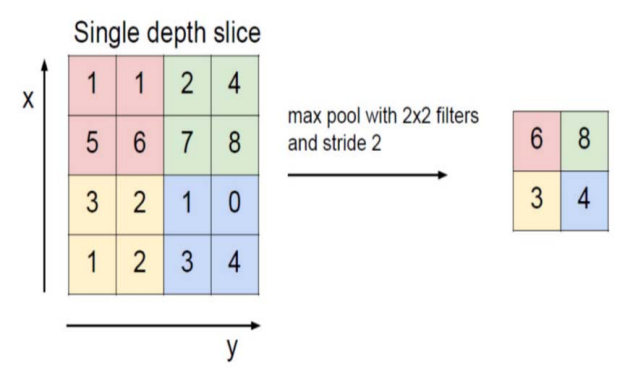
\includegraphics[scale=0.6]{max_pooling.png}
	\caption{Przykładowe działanie max pooling \cite{8308186}}
	\label{max_pooling}
\end{figure}

\subsection{Warstwa Flatten}
\label{flat}

Warstwa \emph{flatten} to warstwa buforowa pomiędzy wielowymiarowymi danymi pochodzącymi z warstw konwolucyjnych i \emph{pooling}, a warstwami klasycznych sieci neuronowych \emph{Dense}. 
\begin{figure}[h]
	\centering
	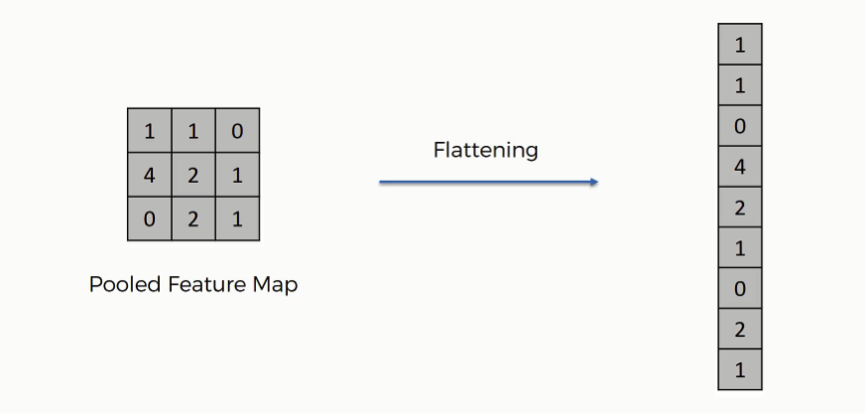
\includegraphics[scale=0.6]{flatten.png}
	\caption{Przykładowe działanie warstwy flatten \cite{superddflatten}}
	\label{flatten}
\end{figure}
Jak nazwa opisywanej warstwy wskazuje - dokonuje ona spłaszczenia wielowymiarowych danych do jednego długiego wektora, który może zostać przekazany do następnych warstw, które na podstawie danych zawartych w tym wektorze sklasyfikują ostateczny wynik \cite{superddflatten}.

Przykład działania warstwy \emph{flatten} został przedstawiony na rysunku \ref{flatten}.



\subsection{Warstwy Dense}
\label{dense}
Warstwy \emph{fully-connected} są podobne do tych znajdujących się w zwykłych sieciach neuronowych. Każdy węzeł jest bezpośrednio połączony z każdym węzłem z poprzedniej i następnej warstwy (rys. \ref{fullycon}) \cite{8308186}. 

\begin{figure}[h]
	\centering
	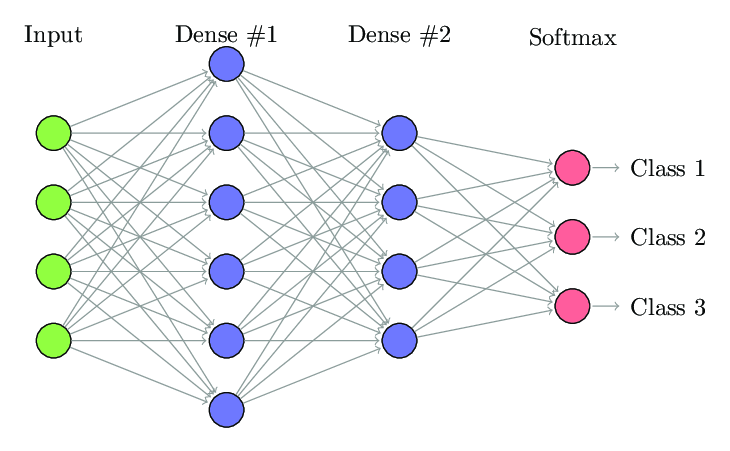
\includegraphics[scale=0.4]{fullycon.png}
	\caption{Przykład warstw \emph{fully-connected} \cite{fullycon}}
	\label{fullycon}
\end{figure}

Przy przetwarzaniu obrazów wprowadzane do sieci są bardzo duże ilości danych. Dzięki sekcji warstw konwolucyjnych i \emph{pooling} następuje redukcja rozmiaru danych jakie trafiają do warstw \emph{fully-connected}. Bez tego przetwarzanie obrazów byłoby niemożliwe lub bardzo wolne z powodu dużego zapotrzebowania warstw \emph{fully-connected} na moc obliczeniową z racji na obecność wielu równoległych obliczeń w tych warstwach \cite{8308186}. 

\section{Zastosowania}

Sieci \emph{CNN} są używane w wielu istniejących aplikacjach. Można ich użyć wszędzie tam gdzie istnieje potrzeba analizy wzorców występujących w tekscie, dzwięku czy oczywiście w obrazach. Najczęstsze zastosowania między innymi to:
\begin{itemize}
	\item rozpoznawanie twarzy,
	\item rozpoznawanie emocji twarzy,
	\item rozpoznawanie obiektów,
	\item autonomiczne pojazdy,
	\item translacja języków,
	\item predykcja następnego słowa na podstawie kontekstu wpisywanego zdania,
	\item rozpoznawanie pisma odręcznego,
	\item analiza obrazów medycznych takich jak zdjęcia rentgenowskie,
	\item wykrywanie nowotworów,
	\item przetwarzanie zapytań w języku naturalnym,
	\item opisywanie obrazów,
	\item uwierzytelnianie na podstawie parametrów biometrycznych,
	\item klasyfikacja dokumentów,
	\item segmentacja trójwymiarowych obrazów medycznych \cite{cnnapps}.
\end{itemize}

Na potrzeby tej pracy w rozdziale \ref{mnist} zostanie przedstawiony przykład klasyfikacji wieloklasowej.

\subsection{MNIST}
\label{mnist}
Zbiór \emph{MNIST} zawiera w sobie 70000 obrazów odręcznie pisanych cyfr z zakresu 0-9. Problem klasyfikacji jest aktualnie przedstawiany jako trywialne i podstawowe zagadnienie w dziedzinie \emph{AI}. Niemniej jednak jest on używany do celów nauki, jak również przez analityków jako próba spekulacji na temat obliczeń sztucznych sieci neuronowych \cite{9388351}. 

Głównym wyzwaniem w zbiorze \emph{MNIST} jest zróżnicowanie odręcznie pisanych cyfr pod względem wielkości, grubości, orientacji i innych czynników. Wynika to z tego, że cyfry były komponowane przez wiele osób z różnymi sposobami pisania \cite{9388351}.
Na rysunku \ref{mnistimg} zostały przedstawione przykładowe cyfry ze zbioru \emph{MNIST}.
\begin{figure}[h]
	\centering
	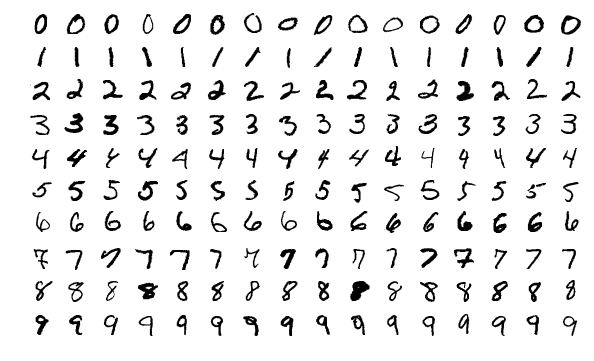
\includegraphics[scale=0.6]{mnistimg.png}
	\caption{Przykłady cyfr ze zbioru \emph{MNIST} \cite{mnistwik}}
	\label{mnistimg}
\end{figure}
Czynnością, od której należy zacząć chcąc pracować z zbiorem \emph{MNIST} jest skorzystanie z interfejsu \emph{Keras API} w celu pobrania zbioru danych. Zbiór \emph{MNIST} jest podzielony na kilka części - część przeznaczoną do treningu modelu i część do ewaluacji stworzonej sieci. Wewnątrz zbiorów treningowych i testowych dane rozdzielone są na obrazy o rozmiarze 28x28 i etykiety, które zawierają numer z zakresu 0-9 odpowiadający cyfrze, do której jest przypisany \cite{mnistapp}. Poszczególne instrukcje zostały przedstawione na listingu \ref{lst:mnistdownload}.

\begin{lstlisting}[language=Python, caption={Pobieranie zbioru \emph{MNIST} \cite{mnistapp}}, label={lst:mnistdownload}]
	import tensorflow as tf
	(x_train, y_train), (x_test, y_test) = tf.keras.datasets.mnist.load_data()
\end{lstlisting}

W celu użycia zbioru danych w modelu niezbędna jest zmiana wymiarów tablic, w~których znajdują się obrazy w celu dodatnia jednego dodatkowego wymiaru. Jest to wymóg użytego API, gdzie ostatni wymiar jest przeznaczony na jedną lub więcej cech danych. Następnie wartości dla poszczególnych pikseli obrazów, które domyślnie znajdują się w zakresie od 0 do 255 muszą zostać znormalizowane do zakresu 0.0-1.0. Najprościej osiągnąć to poprzez operację dzielenia przez 255 wszystkich komórek (listing \ref{lst:mnistreshape}) \cite{mnistapp}.

\begin{lstlisting}[language=Python, caption={Zmiana rozmiarów tablic i normalizacja \cite{mnistapp}}, label={lst:mnistreshape}]
	x_train = x_train.reshape(x_train.shape[0], 28, 28, 1)
	x_test = x_test.reshape(x_test.shape[0], 28, 28, 1)
	input_shape = (28, 28, 1)
	
	x_train = x_train.astype('float32')
	x_test = x_test.astype('float32')
	
	x_train /= 255
	x_test /= 255
\end{lstlisting}

Model do klasyfikacji cyfr na wejściu składa się z jednej warstwy konwolucyjnej posiadającej 28 filtrów i warstwy \emph{MaxPooling}, która zmniejszy rozmiar danych dwukrotnie. Następnie po spłaszczeniu danych do postaci jednowymiarowego wektora, dane przekazywane są do warstw \emph{Dense}, kolejno do warstwy posiadającej 128 węzłów (neuronów) a następnie do warstwy wyjściowej. Warstwa wyjściowa posiada 10 węzłów czyli dokładnie tyle co klas, które model ma przypisywać. Funkcja aktywacji \emph{softmax} pozwoli na odczyt wyników w formie rozkładu prawdopodobieństwa (listing \ref{lst:mnistmodel}) \cite{mnistapp}.

\begin{lstlisting}[language=Python, caption={Budowa modelu \cite{mnistapp}}, label={lst:mnistmodel}]
	from tensorflow.keras.models import Sequential
	from tensorflow.keras.layers import Dense, Conv2D, Dropout, Flatten, MaxPooling2D
	model = Sequential()
	model.add(Conv2D(28, kernel_size=(3,3), input_shape=input_shape))
	model.add(MaxPooling2D(pool_size=(2, 2)))
	model.add(Flatten())
	model.add(Dense(128, activation=tf.nn.relu))
	model.add(Dropout(0.2))
	model.add(Dense(10,activation=tf.nn.softmax))
\end{lstlisting}

\begin{figure}[h]
	\centering
	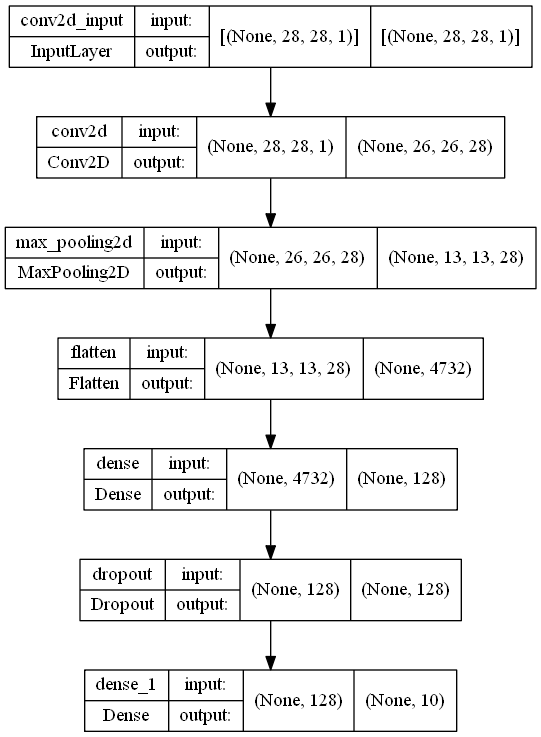
\includegraphics[scale=0.4]{model_plot.png}
	\caption{Wizualizacja modelu}
	\label{model_plot}
\end{figure}

Model stworzony w listingu \ref{lst:mnistmodel} musi zostać skompilowany. Zostaną do niego dodane optymalizator, funkcja straty i metryki. Tak skompilowany model może zostać przedstawiony do treningu (listing \ref{lst:mnisttraining}) \cite{mnistapp}. 

\begin{lstlisting}[language=Python, caption={Kompilacja i trening modelu \cite{mnistapp}}, label={lst:mnisttraining}]
	model.compile(optimizer='adam', loss='sparse_categorical_crossentropy', metrics=['accuracy'])
	model.fit(x=x_train,y=y_train, epochs=10)
\end{lstlisting}

Wytrenowany model może zostać poddany ewaluacji na testowych danych (listing \ref{lst:mnisteval}). Model osiąga wyniki w okolicach 98\%-99\% poprawności klasyfikacji \cite{mnistapp}. 

\begin{lstlisting}[language=Python, caption={Ewaluacja modelu \cite{mnistapp}}, label={lst:mnisteval}]
	model.evaluate(x_test, y_test)
\end{lstlisting}

% chyba mi się nie chce xD
%\subsection{Cats vs Dogs}
%\label{catsdogs}
%\lipsum[1]

\chapter{Implementacja aplikacji do rozpoznawania języka migowego ASL}

Celem niniejszej pracy jest stworzenie aplikacji, która pozwoli na rozpoznawanie części języka ASL - \emph{ASL Manual Alphabet} w czasie rzeczywistym. Program będzie rozpoznawał 26 znaków odpowiadających pojedynczym literom. Aplikacja jako źródło obrazu wykorzystywać będzie kamerę internetową znajdującą się na ekranie monitora. Rozpoznawane znaki będą akceptowane automatycznie przez program i wyświetlane na ekranie po określonej ilości czasu.

\section{Stworzenie zbioru obrazów}

Z racji słabej jakości zbiorów danych dostępnych w ogólnodostępnych źródłach, takich jak portal \emph{Kaggle.com}, na potrzeby tej pracy został stworzony autorski zbiór około 51821 zdjęć przedstawiających 26 znaków z języka \emph{American Sign Language}.

Przeprowadzone testy na zbiorach danych pobranych ze strony z \emph{Kaggle.com} \cite{asl1}\cite{asl2} nie spełniały oczekiwań. Stworzony model miał problemy z treningiem i stabilnością. Było to spowodowane bardzo złą jakością większości zdjęć ze zbioru. Oświetlenie gra kluczową rolę w dziedzinie rozpoznawania obrazu. Wspomniane zdjęcia były w ogólnym pojęciu bardzo ciemne ze względu na prawdopodobny brak jakiegokolwiek źródła światła, a czasem wręcz zdjęcie zostało zrobione "pod" światło (rys. \ref{asl_bad_photo}). 

\begin{figure}[h]
	\centering
	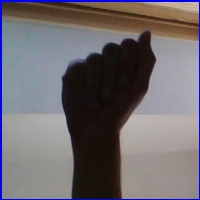
\includegraphics[scale=0.6]{asl_bad_photo.jpg}
	\caption{Słabej jakości zdjęcie znaku ASL ze zbioru danych opublikowanych na \emph{Kaggle.com} \cite{asl1}}
	\label{asl_bad_photo}
\end{figure}

Dobra jakość zdjęcia jest niezbędna przy próbie wykrywania znaków języków migowych. Często znaki te różnią się pozycją jednego palca. Model nie był w stanie zauważyć takich zmian nie widząc wyraźnych krawędzi pomiędzy poszczególnymi częściami dłoni użytkownika.

Ważnym aspektem było też zachowanie realizmu przy tworzeniu zbioru danych. Zdjęcia zawierają nie tylko dłoń na w miarę jednolitym tle, ale również częściowo postać użytkownika i fragmenty niejednolitego otoczenia za nim. Dłoń użytkownika również w realistycznych warunkach będzie znajdowała się w różnych odległościach, pozycjach na ekranie i pod różnymi kontami względem kamery. W takich warunkach model będzie eksploatowany w stworzonej aplikacji więc racjonalnym podejściem było wprowadzić te zmiany już na etapie treningu. 

Przykładowe zdjęcia ze stworzonego zbioru danych znajdują się na rys. \ref{asl_own_photos}.

\begin{figure}[h]
	\centering
		\begin{subfigure}{0.4\textwidth}
			\centering
			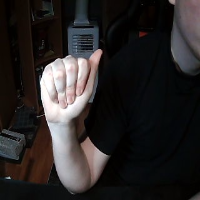
\includegraphics[width=0.7\textwidth]{asl_a.png}
			\caption{A}
		\end{subfigure}
		\begin{subfigure}{0.4\textwidth}
			\centering
			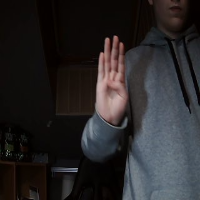
\includegraphics[width=0.7\textwidth]{asl_b.png}
			\caption{B}
		\end{subfigure}
		\begin{subfigure}{0.4\textwidth}
			\centering
			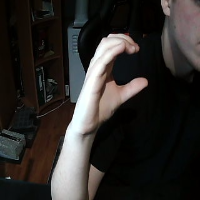
\includegraphics[width=0.7\textwidth]{asl_c.png}
			\caption{C}
		\end{subfigure}
		\begin{subfigure}{0.4\textwidth}
			\centering
			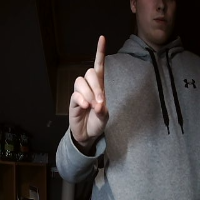
\includegraphics[width=0.7\textwidth]{asl_d.png}
			\caption{D}
		\end{subfigure}
	\caption{Zestawienie przykładowych obrazów z autorskiego zbioru liter języka ASL}
	\label{asl_own_photos}
\end{figure}

\section{Budowa modelu}

Pierwszą czynnością prowadzącą do budowy aplikacji jest przygotowanie danych oraz zbudowanie i wytrenowanie modelu, który będzie wykorzystywany w aplikacji.

Wszystkie wykorzystywane biblioteki do kolejnych podrozdziałów zostały zawarte na listingu \ref{lst:modelimports}.

\begin{lstlisting}[language=Python, caption={Importowane biblioteki}, label={lst:modelimports}]
	# %% Imports
	from pathlib import Path
	
	import cv2
	import matplotlib.pyplot as plt
	import numpy as np
	import tensorflow as tf
	from keras_preprocessing.image import ImageDataGenerator
\end{lstlisting}

Budowa modelu CNN będzie odbywać się z wykorzystaniem biblioteki \emph{Keras}, która znajduje się w bibliotece \emph{tensorflow}. Zawiera ona narzędzia niezbędne do tworzenia, trenowania i wykorzystywania modeli uczenia maszynowego. Dane, których będziemy używać w celu treningu modelu są w formacie zdjęć, więc rozsądnym jest użycie klasy \emph{ImageDataGenerator} z biblioteki \emph{keras\_preprocessing} w celu wygodnego wczytywania obrazów podczas uczenia. 

\subsection{Generatory i argumentacja danych}
Generatory to bardzo popularna metoda wczytywania danych prosto z folderów zawierających zbiór zdjęć. Generator z \emph{Keras API} automatycznie dzieli wczytane obrazy na klasy jeśli są umieszczone w określonej strukturze folderów na dysku \cite{idg}. Pozwalają również na bardzo prostą augmentację danych poprzez różne przekształcenia obrazu, które są losowo aplikowane na wczytywane obrazy. Jest to bardzo dogodne podejście, znacznie wygodniejsze niż wczytywanie wszystkich obrazów do pamięci operacyjnej na raz.

W celu ułatwienia odwoływania się do poszczególnych ścieżek na dysku dobrą praktyką jest zdefiniowanie zmiennych przechowujących te ścieżki za pomocą biblioteki \emph{pathlib} (listing \ref{lst:modelpaths}).

\begin{lstlisting}[language=Python, caption={Definicja ścieżek do danych i modeli}, label={lst:modelpaths}]
	# %% var
	data_path = Path('data/raw')
	train_path = data_path.joinpath('asl-own')
	models_path = Path('models')
\end{lstlisting}

Obiekty generatorów pozwalają na proste podzielenie danych na podzbiory treningowe i walidacyjne. Zbiór walidacyjny posłuży do lepszej oceny sprawności modelu w trakcie uczenia. Oba generatory normalizują wartości pikseli we wczytywanych obrazach do zakresu od 0 do 1 dzięki parametrowi \emph{rescale}. Na danych treningowych w momencie wczytywania zostanie przeprowadzona prosta argumentacja obrazów składająca się z odbicia zdjęć w płaszczyźnie horyzontalnej i losowego przybliżania lub oddalania zdjęcia, w skutek czego sieć neuronowa za każdym razem będzie otrzymywała lekko inny obraz (listing \ref{lst:modelgen}).

\begin{lstlisting}[language=Python, caption={Definicja generatorów}, label={lst:modelgen}]
	# %% generators
	
	data_generator = ImageDataGenerator(
		horizontal_flip=True,
		fill_mode='nearest',
		rescale=1 / 255.0,
		zoom_range=0.2,
		validation_split=0.1
	)
	valid_generator = ImageDataGenerator(
		rescale=1 / 255.0,
		validation_split=0.1
	)
	
	train_gen = data_generator.flow_from_directory(
		directory=train_path,
		target_size=(200, 200),
		color_mode="rgb",
		batch_size=64,
		class_mode="sparse",
		seed=2022,
		subset="training"
	)
	valid_gen = valid_generator.flow_from_directory(
		directory=train_path,
		target_size=(200, 200),
		color_mode="rgb",
		batch_size=64,
		class_mode="sparse",
		seed=2022,
		subset="validation"
	)
	classes = list(train_gen.class_indices.keys())
	print(classes)
	
\end{lstlisting}

Generatory można przetestować ręcznie i wyświetlić wczytywane obrazy w sposób przedstawiony na listingu \ref{lst:modelgentest} za pomocą biblioteki \emph{OpenCV} \cite{opencv}.

\begin{lstlisting}[language=Python, caption={Wczytanie i wyświetlenie pierwszych 10 zdjęć za pomocą ImageDataGenerator}, label={lst:modelgentest}]
	# %% test generators
	def decode_class(cls, one_hot):
		return cls[np.argmax(one_hot)]
		
	for i in range(10):
		image, label = next(train_gen)
		print(decode_class(classes, label))
		image = image[0] * 255.0
		image = image.astype('uint8')
		image = np.squeeze(image)
		cv2.imshow('i', image)
		cv2.waitKey(0)
		cv2.destroyAllWindows()
\end{lstlisting}

Na tym etapie generatory są gotowe do użycia w sieci neuronowej. Użycie klasy \emph{ImageDataGenerator} pozwala na bardzo wygodną augmentację danych i doczytywanie zdjęć w trakcie treningu modelu, a nie wczytania całości zbioru danych do pamięci operacyjnej przed treningiem, co w przypadku większych zbiorów zdjęć byłoby zadaniem niemożliwym z racji ograniczonych zasobów pamięci RAM.

\subsection{Architektura modelu}

Przedstawiony model w listingu \ref{lst:model} i jego struktura została wyłoniona jako najlepsza z testowanych konfiguracji sieci w procesie tworzenia aplikacji. Zastosowane zostały warstwy \emph{Conv2D} występujące w parach, pomiędzy którymi znajduje się warstwa \emph{MaxPooling2D}. Warstwy konwolucyjne posiadają standardowy rozmiar jądra 3x3 i funkcję aktywacji \emph{relu}. W kolejnych warstwach zastosowano rosnącą dwukrotnie, w stosunku do poprzedniej pary, liczbę filtrów.

\begin{lstlisting}[language=Python, caption={Definicja modelu}, label={lst:model}]
	 # %% Build model
	model = tf.keras.models.Sequential()
	model.add(tf.keras.layers.Conv2D(32, (3, 3), activation="relu", padding="same", input_shape=(200, 200, 3)))
	model.add(tf.keras.layers.Conv2D(32, (3, 3), activation="relu", padding="same"))
	model.add(tf.keras.layers.MaxPooling2D(3, 3))
	
	model.add(tf.keras.layers.Conv2D(64, (3, 3), activation="relu", padding="same"))
	model.add(tf.keras.layers.Conv2D(64, (3, 3), activation="relu", padding="same"))
	model.add(tf.keras.layers.MaxPooling2D(3, 3))
	
	model.add(tf.keras.layers.Conv2D(128, (3, 3), activation="relu", padding="same"))
	model.add(tf.keras.layers.Conv2D(128, (3, 3), activation="relu", padding="same"))
	model.add(tf.keras.layers.MaxPooling2D(3, 3))
	
	model.add(tf.keras.layers.Conv2D(256, (3, 3), activation="relu", padding="same"))
	model.add(tf.keras.layers.Conv2D(256, (3, 3), activation="relu", padding="same"))
	
	model.add(tf.keras.layers.Flatten())
	
	model.add(tf.keras.layers.Dense(1500, activation="relu"))
	model.add(tf.keras.layers.Dropout(0.5))
	
	model.add(tf.keras.layers.Dense(26, activation="softmax"))
	
	opt = tf.keras.optimizers.Adam(learning_rate=0.0001)
	model.compile(optimizer=opt, loss="sparse_categorical_crossentropy", metrics=['accuracy'])
	model.summary()
\end{lstlisting}

Stworzony model charakteryzuje się wysoką liczbą (20 028 782) trenowalnych parametrów, głównie z powodu dużej liczby połączeń w przedostatniej warstwie (listing \ref{lst:modelsum}). Pomimo znacznej liczby parametrów model jest wystarczająco szybki aby przetwarzać w czasie rzeczywistym obraz z kamery.

\begin{lstlisting}[language=Python, caption={Podsumowanie modelu}, label={lst:modelsum}]
	Model: "sequential"
	_________________________________________________________________
	Layer (type)                Output Shape              Param #   
	=================================================================
	conv2d (Conv2D)             (None, 200, 200, 32)      896       
	
	conv2d_1 (Conv2D)           (None, 200, 200, 32)      9248      
	
	max_pooling2d (MaxPooling2D  (None, 66, 66, 32)       0         
	)                                                               
	
	conv2d_2 (Conv2D)           (None, 66, 66, 64)        18496     
	
	conv2d_3 (Conv2D)           (None, 66, 66, 64)        36928     
	
	max_pooling2d_1 (MaxPooling  (None, 22, 22, 64)       0         
	2D)                                                             
	
	conv2d_4 (Conv2D)           (None, 22, 22, 128)       73856     
	
	conv2d_5 (Conv2D)           (None, 22, 22, 128)       147584    
	
	max_pooling2d_2 (MaxPooling  (None, 7, 7, 128)        0         
	2D)                                                             
	
	conv2d_6 (Conv2D)           (None, 7, 7, 256)         295168    
	
	conv2d_7 (Conv2D)           (None, 7, 7, 256)         590080    
	
	flatten (Flatten)           (None, 12544)             0         
	
	dense (Dense)               (None, 1500)              18817500  
	
	dropout (Dropout)           (None, 1500)              0         
	
	dense_1 (Dense)             (None, 26)                39026     
	
	=================================================================
	Total params: 20,028,782
	Trainable params: 20,028,782
	Non-trainable params: 0
	_________________________________________________________________
	
\end{lstlisting}

\subsection{Trening modelu}

Trening modelu przebiega w oparciu o zatrzymywanie procesu uczenia na podstawie wyników poszczególnych epok. W wypadku, gdy model zaczyna się przetrenowywać uczenie modelu jest zatrzymywane. Innym równie ważnym czynnikiem jest mechanizm \emph{ModelCheckpoint}. Pozwala on na zapisywanie obiektu modelu po każdej epoce treningu w celu późniejszego wczytania najlepszej wersji.

\begin{lstlisting}[language=Python, caption={Trening modelu i mechanizmy \emph{Callback}}, label={lst:modeltrain}]
	# %% Fit
	model_checkpoint_callback = tf.keras.callbacks.ModelCheckpoint(
		# tekst formatujacy nazwe pliku do ktorego zapisywany jest model
		filepath=models_path.joinpath('{epoch:02d}-{val_loss:.2f}.hdf5'), 
		# zapisz caly model
		save_weights_only=False,
		monitor='val_accuracy', 
		mode='max',
		# zapisz kazdy model
		save_best_only=False)
	
	history = model.fit(train_gen,
		epochs=999,
		validation_data=valid_gen,
		# dodanie wczesniej utworzonego mechanizmu ModelCheckpoint do zapisywania modelu i EarlyStopping do zatrzymywania treningu po spadku precyzji
		callbacks=[model_checkpoint_callback, tf.keras.callbacks.EarlyStopping(patience=2)],
		# liczba procesow uzywanych do wczytywania obrazow
		workers=20)
	
\end{lstlisting}

Model bardzo szybko osiąga dosyć wysoki wynik powyżej 90\%. Po czwartej epoce model zaczyna się przetrenowywać i dokładność na zbiorze walidacyjnym spada. Z danej sesji treningowym najlepszym modelem będzie model zapisany po 4 epoce.

\begin{lstlisting}[language=Python, caption={Przykładowy trening modelu}, label={lst:modeltrainsession}]
	729/729 [==============================] - 108s 138ms/step - loss: 1.0876 - accuracy: 0.6626 - val_loss: 0.4911 - val_accuracy: 0.8657
	Epoch 2/999
	729/729 [==============================] - 133s 179ms/step - loss: 0.1650 - accuracy: 0.9452 - val_loss: 0.4953 - val_accuracy: 0.8691
	Epoch 3/999
	729/729 [==============================] - 126s 171ms/step - loss: 0.0786 - accuracy: 0.9738 - val_loss: 0.3581 - val_accuracy: 0.9114
	Epoch 4/999
	729/729 [==============================] - 124s 168ms/step - loss: 0.0497 - accuracy: 0.9839 - val_loss: 0.3348 - val_accuracy: 0.9203
	Epoch 5/999
	729/729 [==============================] - 108s 145ms/step - loss: 0.0386 - accuracy: 0.9871 - val_loss: 0.3579 - val_accuracy: 0.9043
	...
\end{lstlisting}

Na wykresie \ref{model_train} został zwizualizowany proces treningu i towarzyszące mu parametry dokładności i straty dla danych treningowych i walidacyjnych.

Średni czas potrzebny na trening modelu wynosił od 6 do 10 minut. Model był trenowany na komputerze posiadającym procesor Intel Core i9 10850K na fabrycznym taktowaniu rdzeni oraz wykorzystywał układ GPU - Nvidia RTX 3080. W celu trenowania modelu z wykorzystaniem karty graficznej zainstalowane zostało oprogramowanie \emph{Nvidia Cuda}, które jest wykorzystywane w celu przeprowadzania obliczeń na procesorach graficznych Nvidia \cite{cuda}.

\begin{figure}[h]
	\centering
	\hspace*{-3cm} 
	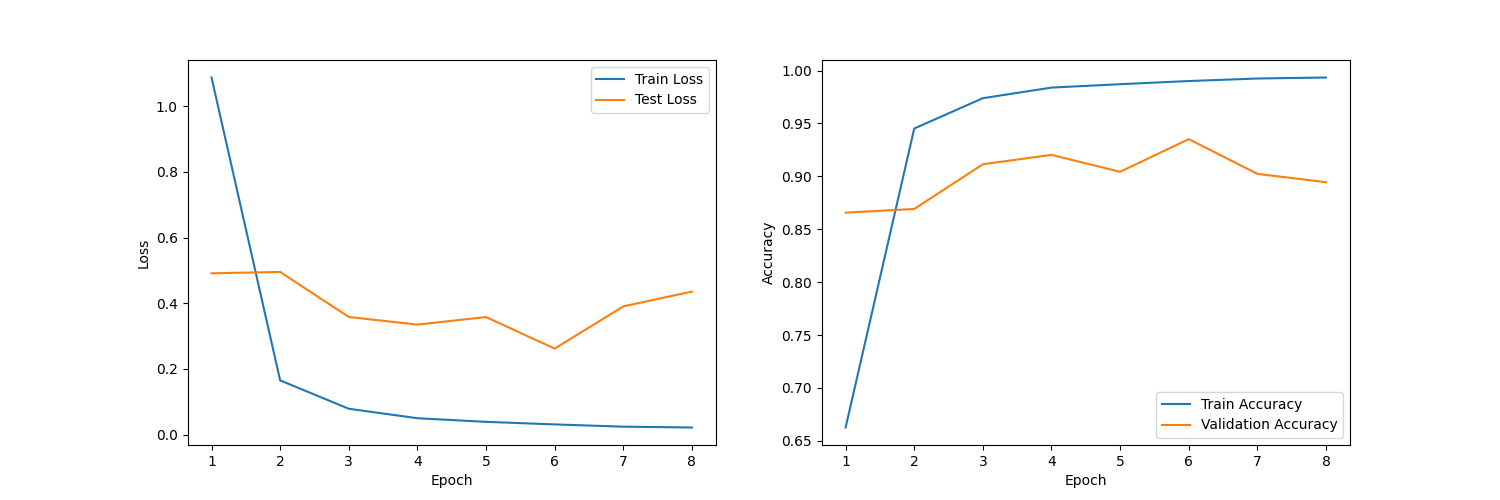
\includegraphics[scale=0.4]{train.png}
	\caption{Wizualizacja treningu}
	\label{model_train}
\end{figure}

\section{Aplikacja do rozpoznawania języka migowego w czasie rzeczywistym}

W ramach niniejszej pracy licencjackiej powstała aplikacja rozpoznająca znaki języka ASL w czasie rzeczywistym, stanowiąca niejako studium wykonalności. Aplikacja z dobrze wytrenowanym modelem jest w stanie w czasie rzeczywistym z dużą skutecznością rozpoznawać znaki pokazywane przez użytkownika.

W celu implementacji skorzystano z bibliotek \emph{OpenCV}, \emph{Tensorflow}, \emph{numpy} i \emph{time}. Przed wystąpieniem głównej pętli programowej inicjalizowane są zmienne odpowiadające za między innymi interfejs kamery i wczytany model. Metoda \emph{decode\_class} odpowiada za translację wektora zwracanego przez model na konkretną literę alfabetu (listing \ref{lst:appimports}).

\begin{lstlisting}[language=Python, caption={Wykorzystywane biblioteki i inicjalizacja zmiennych}, label={lst:appimports}]
	import cv2
	import numpy as np
	import tensorflow as tf
	import time
	
	vid = cv2.VideoCapture(0)
	vid.set(cv2.CAP_PROP_FRAME_WIDTH, 200)
	vid.set(cv2.CAP_PROP_FRAME_HEIGHT, 200)

	model = tf.keras.models.load_model('models/04-0.34.hdf5')
	
	def decode_class(one_hot):
		cls = ['A', 'B', 'C', 'D', 'E', 'F', 'G', 'H', 'I', 'J', 'K', 'L', 'M', 'N', 'O', 'P', 'Q', 'R', 'S', 'T', 'U', 'V', 'W', 'X', 'Y', 'Z']
		return cls[np.argmax(one_hot)]
	
	last_char = 'None'
	text = ''
	char_time_start = time.time()
\end{lstlisting}

Główna pętla programowa zajmuje się pozyskiwaniem klatek z kamery za pomocą metody \emph{vid.read()}. Tak pozyskana klatka jest zmniejszana do rozmiaru 200x200 pikseli i normalizowana w celu klasyfikacji przez model. Następnie wynik klasyfikacji jest dekodowany wcześniej wspomnianą metodą \emph{decode\_class} dla otrzymania konkretnej litery. Litera jest akceptowana i wyświetlana na ekranie jeśli występuje niezmiennie przez określoną ilość czasu.

\begin{lstlisting}[language=Python, caption={Pętla programowa}, label={lst:apploop}]
	while True:
		ret, frame = vid.read()
		batch = cv2.resize(frame, (200, 200))
		batch = np.reshape(batch, (1, 200, 200, 3))
		batch = batch * (1 / 255.)
		pred = model.predict(batch, verbose=0)
		char = decode_class(pred)
		if char != last_char:
			last_char = char
			char_time_start = time.time()
		if (time.time() - char_time_start) > 2.0:
			text += char
			char_time_start = time.time()
		frame = cv2.putText(frame,
			f'Char: {char}',
			org=(1, 30),
			fontFace=cv2.FONT_HERSHEY_SIMPLEX,
			fontScale=1,
			thickness=1,
			color=(0, 0, 255))
		frame = cv2.putText(frame,
			f'Text:{text if len(text) < 10 else text[-10:]}',
			org=(1, 55),
			fontFace=cv2.FONT_HERSHEY_SIMPLEX,
			fontScale=1,
			thickness=1,
			color=(0, 255, 0))
		cv2.imshow('frame', frame)
		key = cv2.waitKey(1) & 0xFF
		if key == ord('a'):
			text += char
			char_time_start = time.time()
		if key == ord('s'):
			text = text[:-1]
		if key == ord('q'):
			break
	vid.release()
	cv2.destroyAllWindows()
\end{lstlisting}

Praktyczne działanie programu przedstawia rys. \ref{umcs}. W danym przypadku udało się pomyślnie wypisać na ekranie skrót nazwy Uniwersytetu Marii Curie-Słodowskiej.

\begin{figure}[h]
	\centering
	\begin{subfigure}{0.4\textwidth}
		\centering
		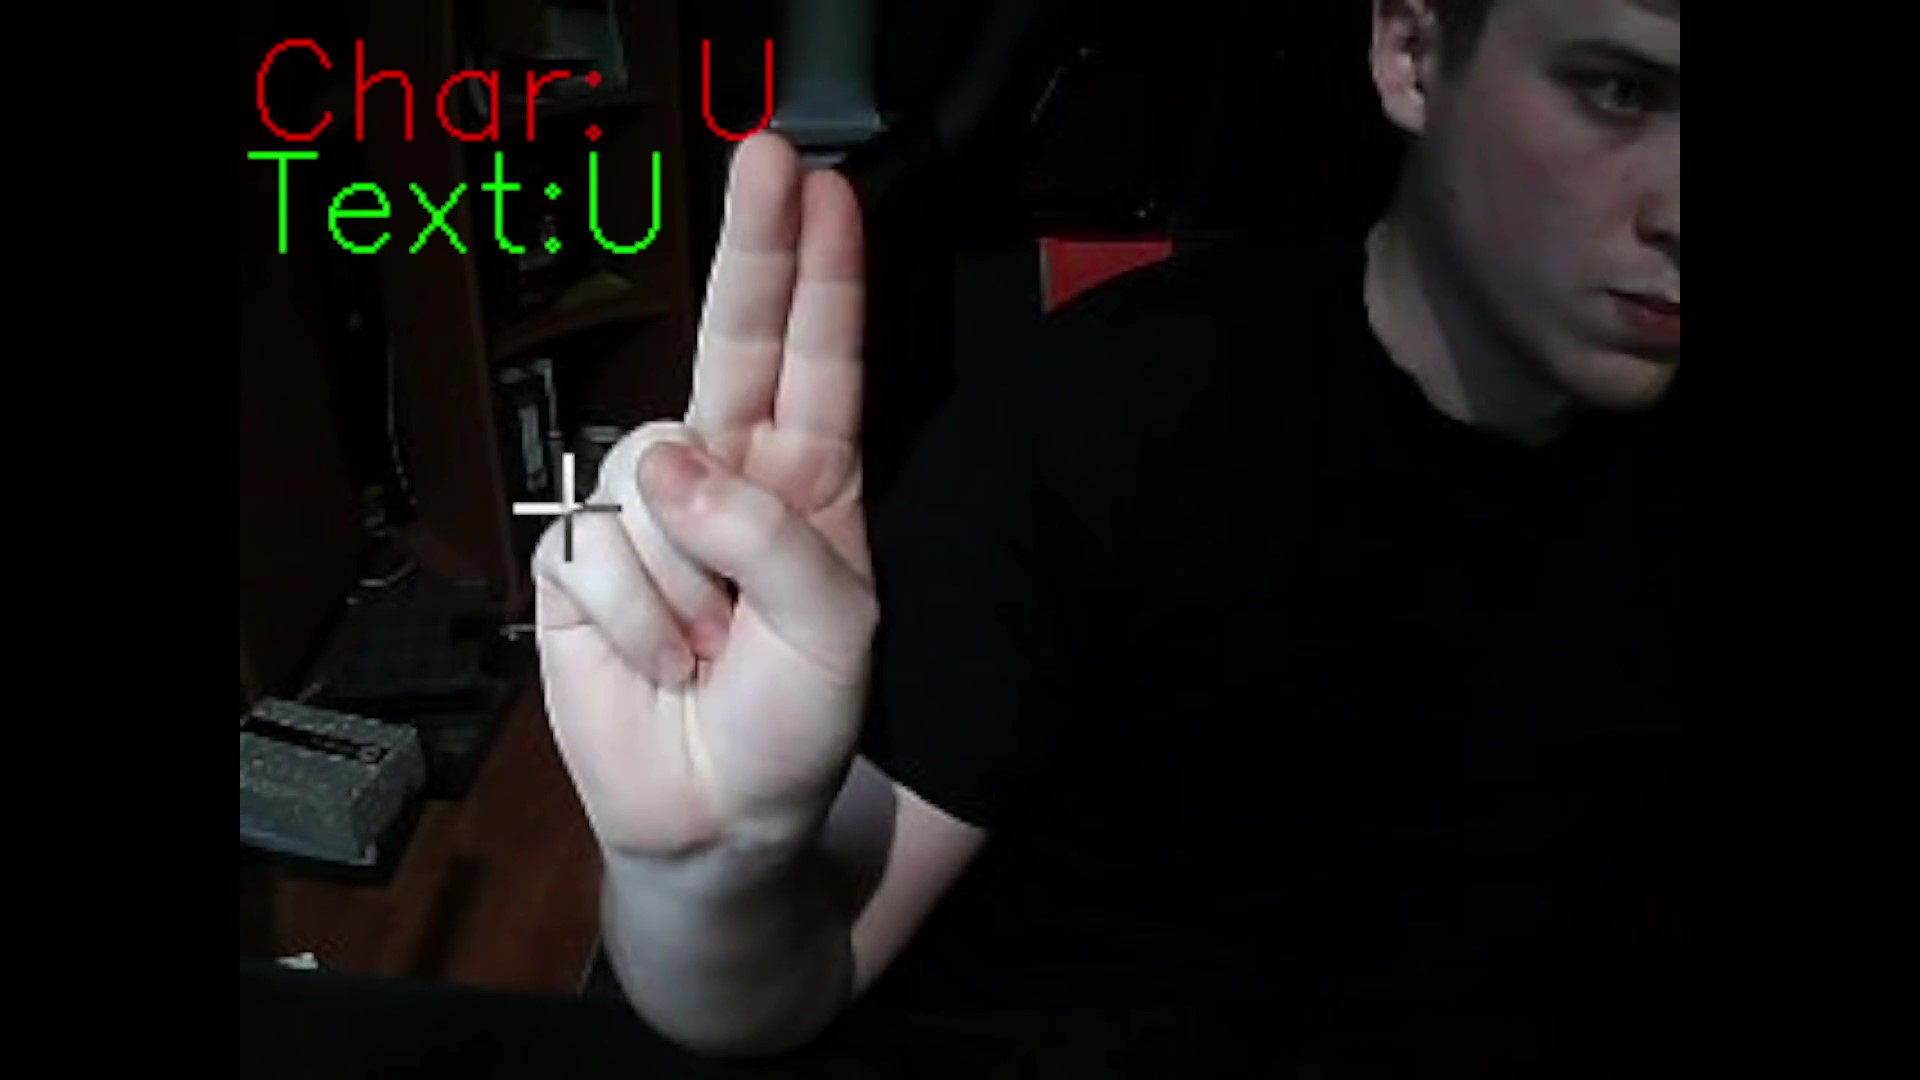
\includegraphics[width=0.95\textwidth]{U.jpg}
	\end{subfigure}
	\begin{subfigure}{0.4\textwidth}
		\centering
		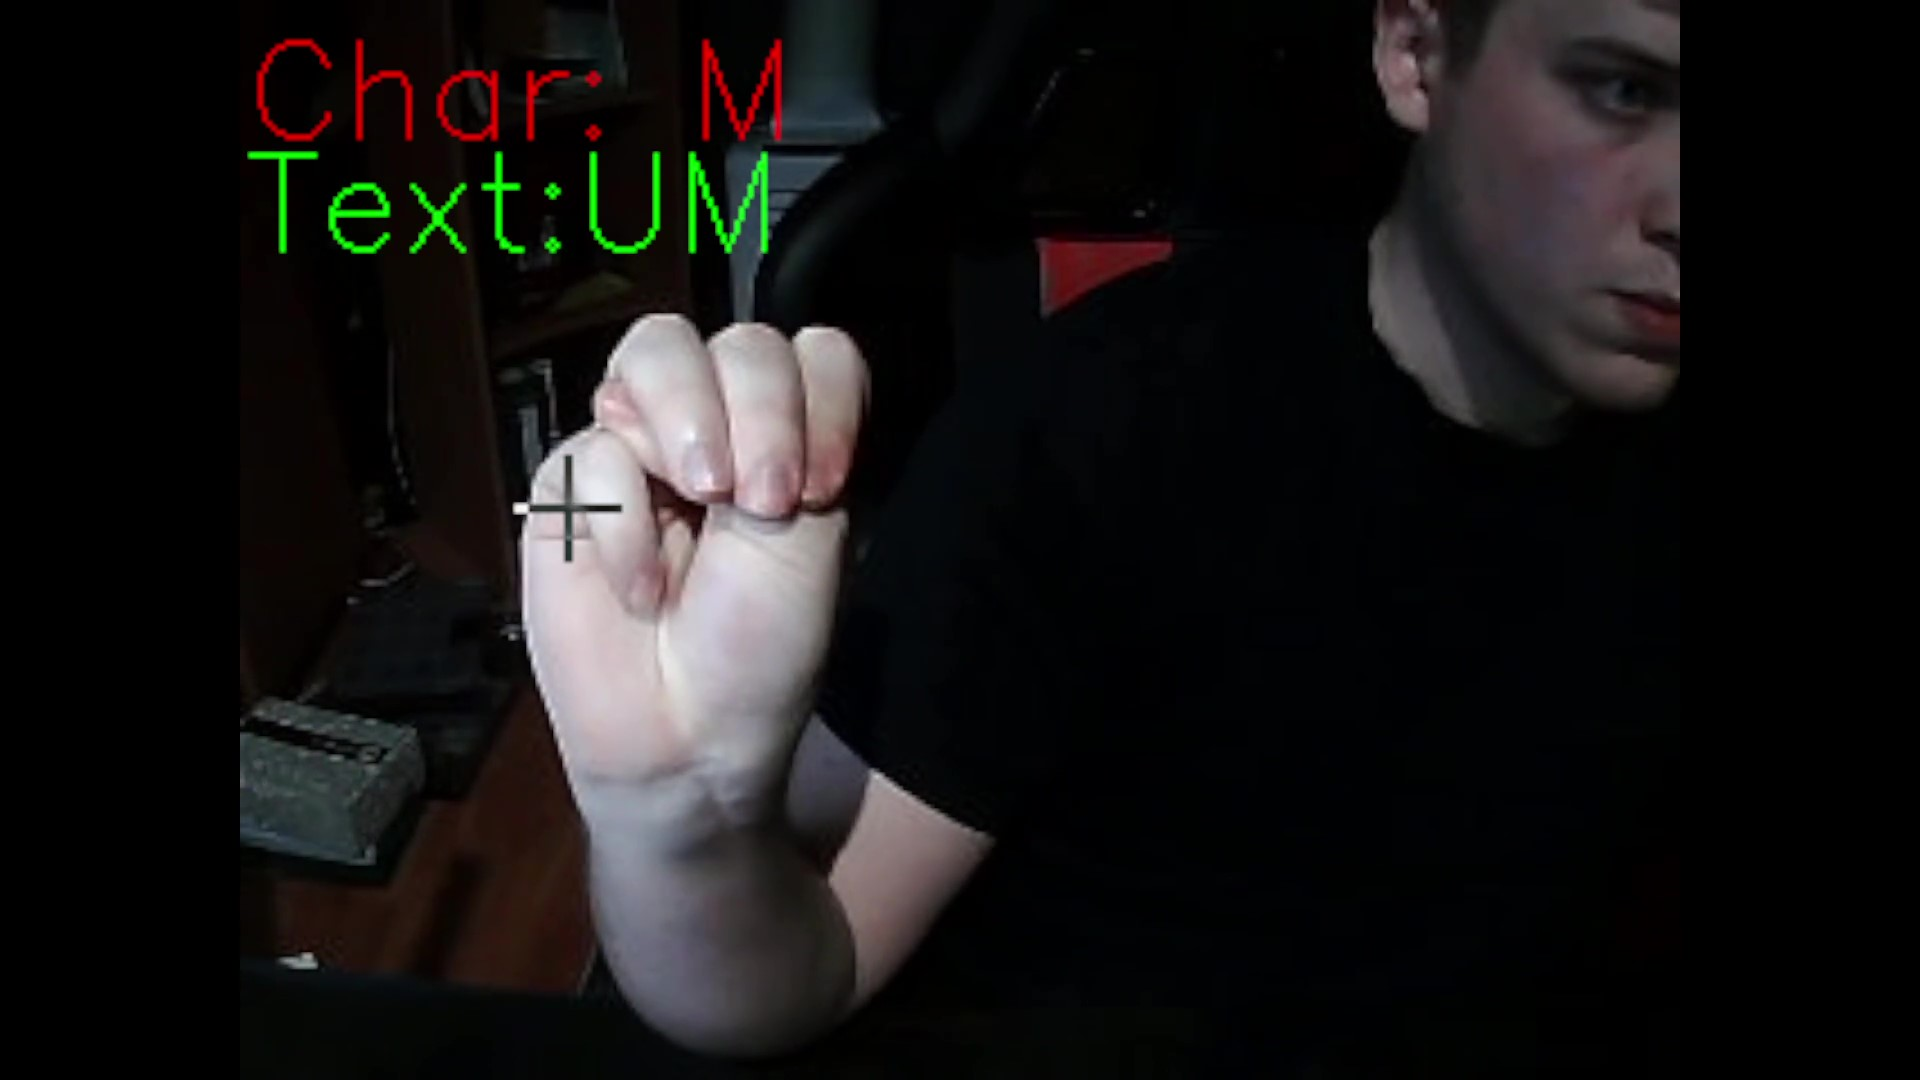
\includegraphics[width=0.95\textwidth]{UM.jpg}
	\end{subfigure}
	\begin{subfigure}{0.4\textwidth}
		\centering
		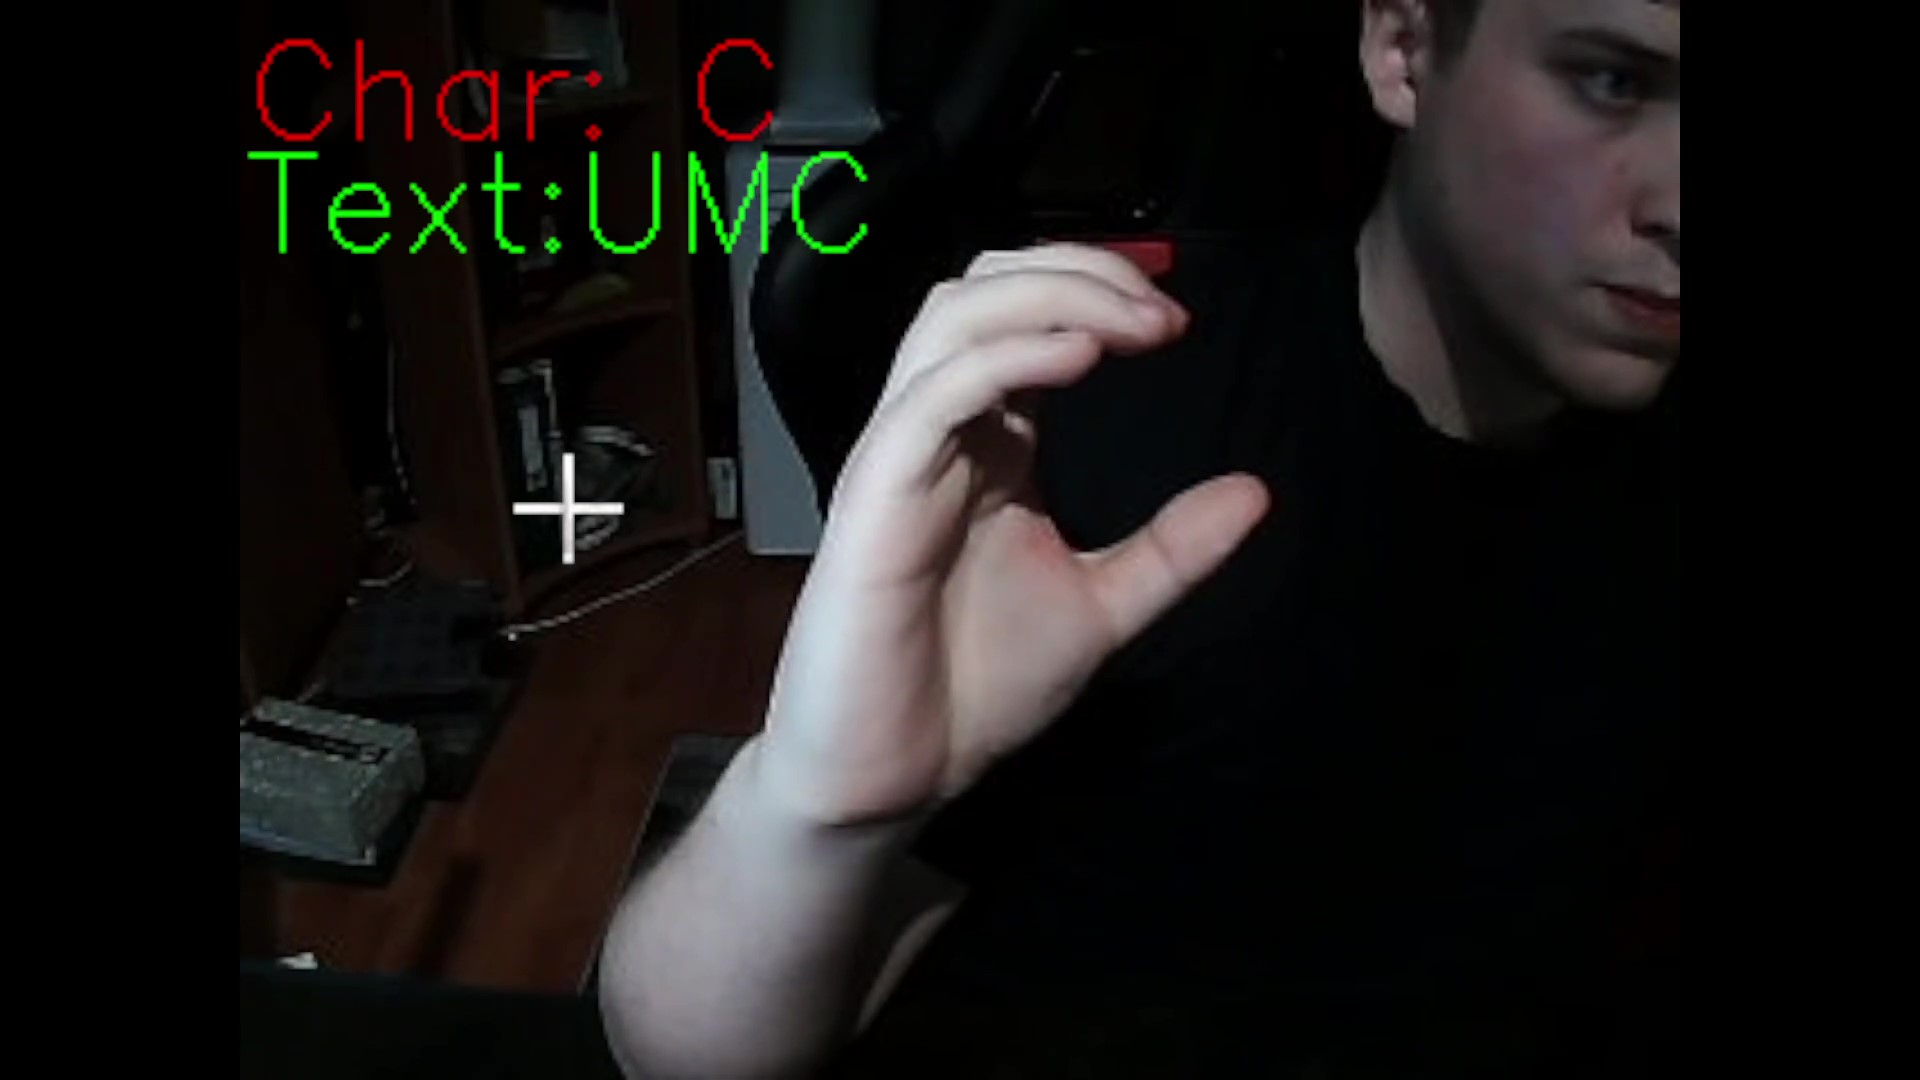
\includegraphics[width=0.95\textwidth]{UMC.jpg}
	\end{subfigure}
	\begin{subfigure}{0.4\textwidth}
		\centering
		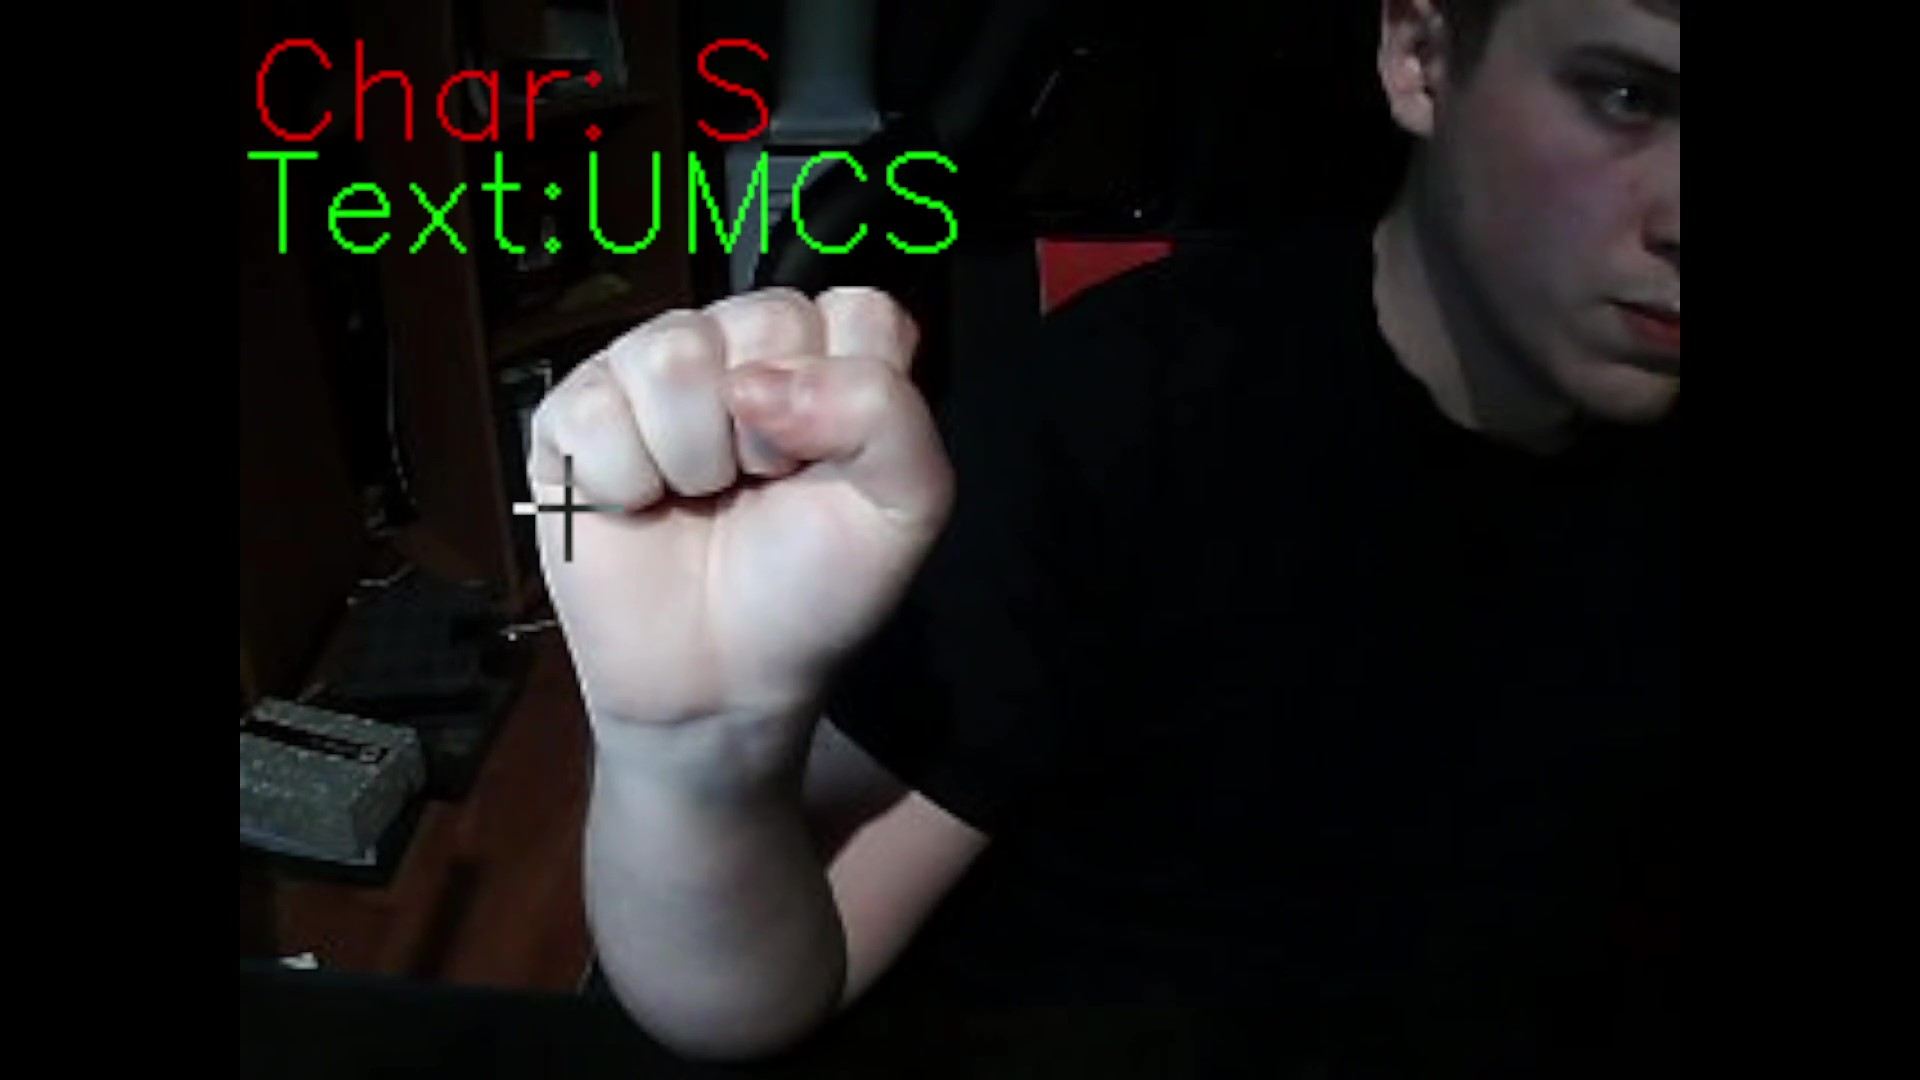
\includegraphics[width=0.95\textwidth]{UMCS.jpg}
	\end{subfigure}
	\caption{Praktyczne działanie programu}
	\label{umcs}
\end{figure}

\section{Analiza błędów}

Aplikacja pomimo odpowiednio przygotowanych zdjęć i dobrego oświetlenia ma problemy z rozróżnianiem znaków języka migowego odpowiadającym literom "m", "n", "s", "t" i czasami "a". Wynika to z podobieństwa układów dłoni i palców reprezentujących te litery. We wszystkich przypadkach jest to zaciśnięta pięść, gdzie czynnikiem determinującym konkretną literę jest pozycja kciuka - na zewnątrz pięści, wewnątrz lub pomiędzy którymi palcami się on znajduje, przykładowo tak jak w znakach odpowiadającym literom "m", "n" i "t".

Rozwiązanie tego problemu może mieć wiele składowych. Przede wszystkim zwiększenie ilości danych w zbiorze zdjęć mogłoby mieć znaczący wpływ na izolację wykrywania znaków języka migowego od czynników otoczenia występujących w polu widzenia kamery. Zbiór danych powinien zostać rozszerzony o nowe otoczenia i aktorów. Również duże znaczenie mogłaby wnieść zmiana rozdzielczości obrazów jakie sieć przyjmuje z 200x200 pikseli na wartości wyższe (400x400, 600x600 i tym podobne). Zmiana rozdzielczości obrazu powiększyłaby liczbę szczegółów widocznych na obrazie co ułatwiłoby klasyfikację modelu.

\chapter{Podsumowanie}

Sieci konwolucyjne to bez wątpienia bardzo dobre narzędzie do analizy i klasyfikacji obrazów. Sposób w jaki sieci konwolucyjne są budowane znacznie zmniejsza zapotrzebowanie na moc obliczeniową w porównaniu do zwykłych sieci neuronowych. Pozwala to stosować modele w aplikacjach wymagających czasu reakcji niemalże w czasie rzeczywistym. Rozpoznawanie języka migowego jest bardzo wymagającym zadaniem, nie jest jednak zadaniem niemożliwym. Przy dzisiejszym postępie technologicznym w dziedzinie sztucznych sieci neuronowych możliwe jest niewielkim nakładem pracy stworzenie modelu oraz aplikacji, które w zadowalający sposób poradzą sobie z problemem klasyfikacji znaków języka migowego.

\listoftables{} % jeśli są tabele
\addcontentsline{toc}{chapter}{Spis tabel}

\listoffigures{} % jeśli są obrazki
\addcontentsline{toc}{chapter}{Spis rysunków}

\lstlistoflistings
\addcontentsline{toc}{chapter}{Spis listingów}

\addcontentsline{toc}{chapter}{Bibliografia}
\bibliographystyle{ieeetr}
\bibliography{bibliography/cite}


\end{document}
